\documentclass[border=0.2cm]{standalone}

%\usepackage[utf8]{inputenc}

%\usepackage{pgffor}
\usepackage{tikz}
\usetikzlibrary{shapes,positioning}

\title{Directed Acyclic Graph}
\date{}


\begin{document}
\maketitle
What's the Use
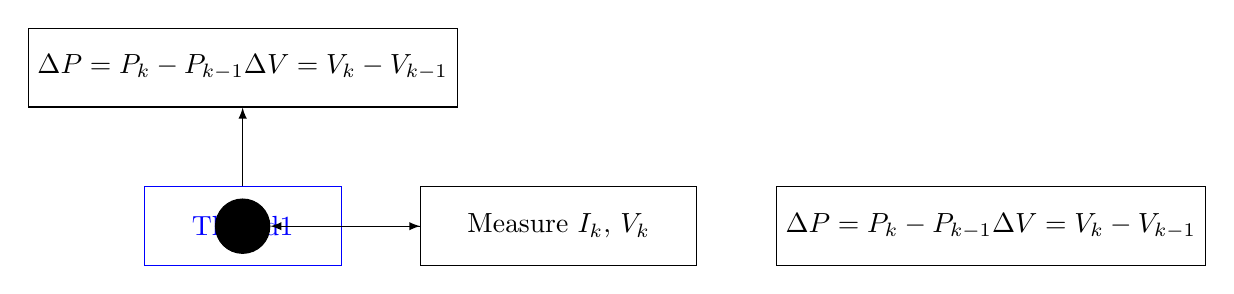
\begin{tikzpicture}
    
% Start block
\node[draw,
    minimum width=2.5cm,
    minimum height=1cm,color=blue] (block1) {Thread1};
 
% Vo Measurement
\node[draw,
    right=of block1,
    minimum width=3.5cm,
    minimum height=1cm
] (block2) { Measure $I_k$, $V_k$ };


\node[draw,
    below=of block2,
    minimum width=3.5cm,
    minimum height=1cm,
    above=of block1
] (block3) { $\Delta P=P_k-P_{k-1}$ \\ $\Delta V=V_k-V_{k-1}$};


\node[draw,
    below=of block2,
    minimum width=3.5cm,
    minimum height=1cm,
    right=of block2
] (block4) { $\Delta P=P_k-P_{k-1}$ \\ $\Delta V=V_k-V_{k-1}$};
 
% Conditions test

 
% Return block
\node[draw,circle,fill=black, minimum size=0.1, inner sep=0pt](circle1) {Join};
 
% Arrows
\draw[-latex] (block1) edge (block2)
    (block1) edge (block3)
    (block2) edge (circle1);

\end{tikzpicture}



%   \begin{circuitikz}
      


%     \begin{scope}[yshift=\n cm]
%          \draw (5,5)--(5,4)to[R,l=R\n](3,4)--(3,5);
         
%     \end{scope}
%     }
%     \foreach \n in {249,250}
%     {
%     begin{scope}[yshift=4 cm]
%     \draw(5,5)--(5,10+\n-250)to[R,l=R\n](3,10+\n-250)--(3,5);
%     }
%     \begin{scope}
    
%     \end{scope}
%     %\end{scope}
%     %\begin{scope}[yshift=0cm]
%      %    \draw(4,5)--(4,4)to[R,l=R](1,4)--(1,5);
%     %\end{scope}
%     %\begin{scope}
     
%     %\end{scope}
%     %\begin{scope}[yshift=0cm]
%      %    \draw(4,5)--(4,6)to[R,l=R](1,6)--(1,5);
%    %\end{scope}
 
%    \draw
%    (3,5)--(0,5)
%    (0,5)--(0,0);
       
 
%  \end{circuitikz}

\end{document}